%%\section{モジュール仕様書}

設計した各モジュールについて,上位階層から順にモジュールの仕様を示す.

\subsection{Golden\_Top}
このモジュールは最上位に位置し,
コンパイル時に\texttt{IMem.txt}に書き込まれた命令をボタン押下に応じて順に実行する.
現在のプログラムカウンタや内部モジュールの出力を7セグLEDで表示し,
命令の実行結果が確認できるように構成している.

デフォルトで定義されているクロックやGPIOの定義に加え,以下のモジュールをインスタンス化する.
モジュール名とインスタンス名を表\ref{tab:golden_top_mod}に示す.
\begin{table}[h]
  \centering
  \caption{Golden\_Top で利用するモジュール}
  \begin{tabular}{l|l}
    モジュール名 & インスタンス名 \\
    \hline
    BTN\_IN & BTN0 \\
    SingleCycleClockMIPS & SCCM0 \\
    SELECTOR & SEL0 \\
    SEG7DEC & Res00 \\
    SEG7DEC & Res01 \\
    SEG7DEC & Res02 \\
    SEG7DEC & Res03 \\
    SEG7DEC & PC00 \\
    SEG7DEC & PC01
  \end{tabular}
  \label{tab:golden_top_mod}
\end{table}
上記のモジュールの接続関係を図\ref{fig:golden_top_block}に示す.
\begin{figure}[h]
  \centerning
  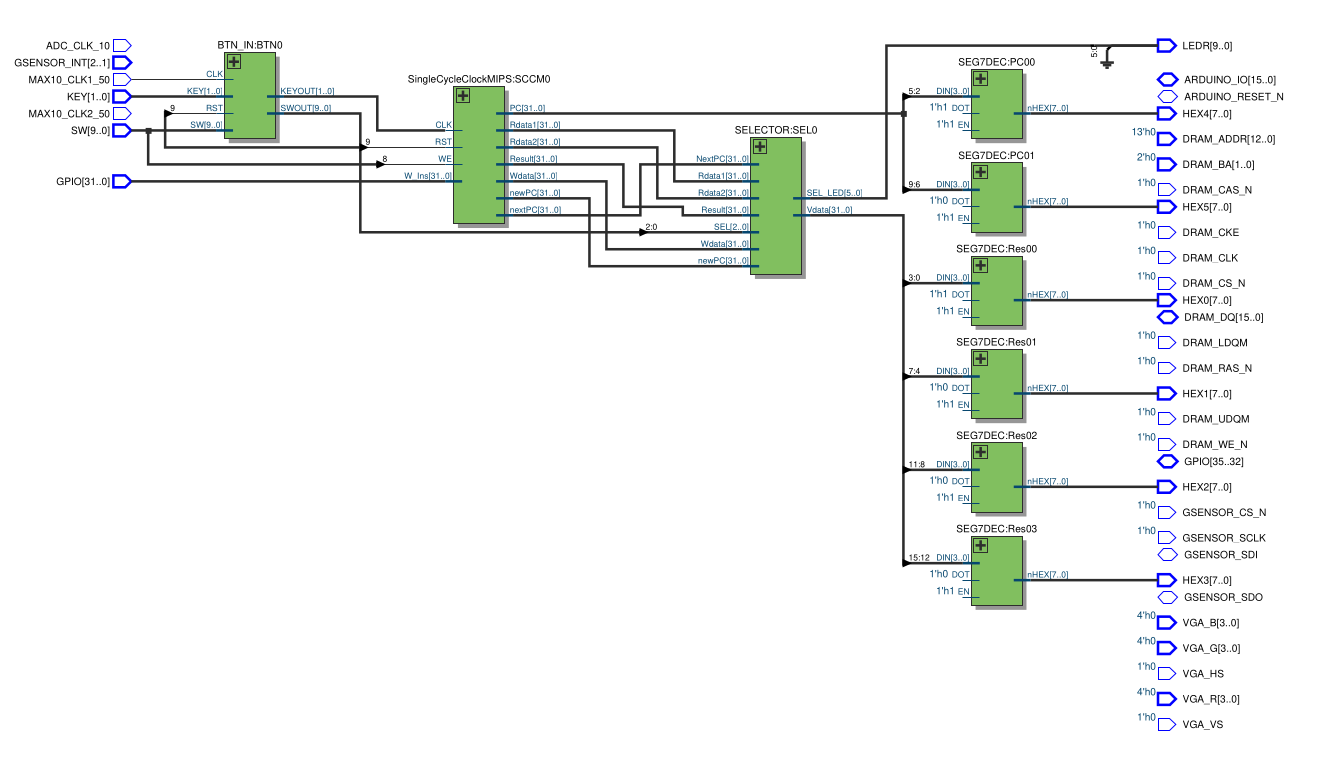
\includegraphics[width=\textwidth]{myRTL.png}
  \caption{Golden\_Top のサブモジュール間の接続関係}
  \label{fig:golden_top_block}
\end{figure}

\subsection{BTN\_IN}
このモジュールは Golden\_Top 内で利用されており,
DE10-lite の KEY 及び SW から得られる入力のチャタリングを排除し,
KEY は立下がりを検出する.
本モジュールの入力・出力信号を表\ref{tab:btn_in_input}, \ref{tab:btn_in_output}に示す.
\begin{table}[h]
  \caption{BTN\_IN の入力信号}
  \centering
  \begin{tabular}{l|l|l}
    信号名 & ビット幅 & 説明 \\
    \hline
    CLK & [0:0] & DE10-lite で生成するクロック信号 \\
    RST & [0:0] & リセット用信号 (DE10-lite の SW9) \\
    KEY & [1:0] & DE10-lite の KEY 入力信号 \\
    SW &  [9:0] & DE10-lite の SW 入力信号
  \end{tabular}
  \label{tab:btn_in_input}
\end{table}
\begin{table}[h]
  \caption{BTN\_IN の出力信号}
  \centering
  \begin{tabular}{l|l|l}
    信号名 & ビット幅 & 説明 \\
    \hline
    KEYOUT & [1:0] & チャタリングを排除したKEYの立下がりレジスタ値 \\
    SWOUT &  [9:0] & チャタリングを排除したSWのレジスタ値
  \end{tabular}
  \label{tab:btn_in_output}
\end{table}

チャタリングを排除するために,40hz毎に入力信号KEY, SWの値を読み出す.
このとき,入力を読み出すフリップフロップ(FF)と直前の値を読み出すFF2個を用いる.
入力ではなく直前の値を利用することで,チャタリング排除する.
同期回路でチャタリングを排除した信号を出力する.


\subsection{SingleCycleClockMIPS}
このモジュールは Golden\_Top 内で利用されており,
コンパイル時に\texttt{IMem.txt}で指定された命令を実行するシングルサイクルクロックのMIPSである.
動作クロックは,DE10-lite の KEY0 とする.
本モジュールの入力・出力信号を表\ref{tab:sccm_input}, \ref{tab:sccm_output}に示す.
\begin{table}[h]
  \caption{SingleCycleClockMIPS の入力}
  \centering
  \begin{tabular}{l|l|l}
    信号名 & ビット幅 & 説明 \\
    \hline
    CLK & [0:0] & SingleCycleClockMIPS 用のクロック信号 \\
    RST & [0:0] & リセット用信号 \\
    WE & [0:0] & コンパイル時にIFモジュールの最適化を防止するための信号 \\
    W\_Ins & [31:0] & コンパイル時にIFモジュールの最適化を防止するための信号 \\
  \end{tabular}
  \label{tab:sccm_input}
\end{table}
\begin{table}[h]
  \caption{SingleCycleClockMIPS の出力}
  \centering
  \begin{tabular}{l|l|l}
    信号名 & ビット幅 & 説明 \\
    \hline
    PC & [31:0] & 今から実行する命令のアドレスを示す値 \\
    Result & [31:0] & EXモジュールで出力するALUの結果を示す値 \\
    Rdata1 & [31:0] & IDモジュールで出力,IFモジュールで入力される値 \\
    Rdata2 & [31:0] & IDモジュールで出力,IF・MAモジュールで入力される値 \\
    Wdata & [31:0] & MAモジュールで出力,IDモジュールで入力される値 \\
    nextPC & [31:0] & PC に 4 を加えた値 \\
    newPC & [31:0] & EXモジュールで決定する次の命令アドレスを示す値 \\
  \end{tabular}
  \label{tab:sccm_output}
\end{table}

本モジュールでは表\ref{tab:sccm_mod}のサブモジュールを利用する.
また,サブモジュール間の接続関係を図\ref{fig:sccm_mod}に示す.
\begin{table}[h]
  \caption{SingleCycleClockMIPS で用いるサブモジュール}
  \centering
  \begin{tabular}{l|l}
    モジュール名 & インスタンス名 \\
    \hline
    IF & IF0 \\
    ID & ID0 \\
    EX & EX0 \\
    MA & MA0 \\
  \end{tabular}
  \label{tab:sccm_mod}
\end{table}
\begin{figure}
  \centering
  %% wip
  %% 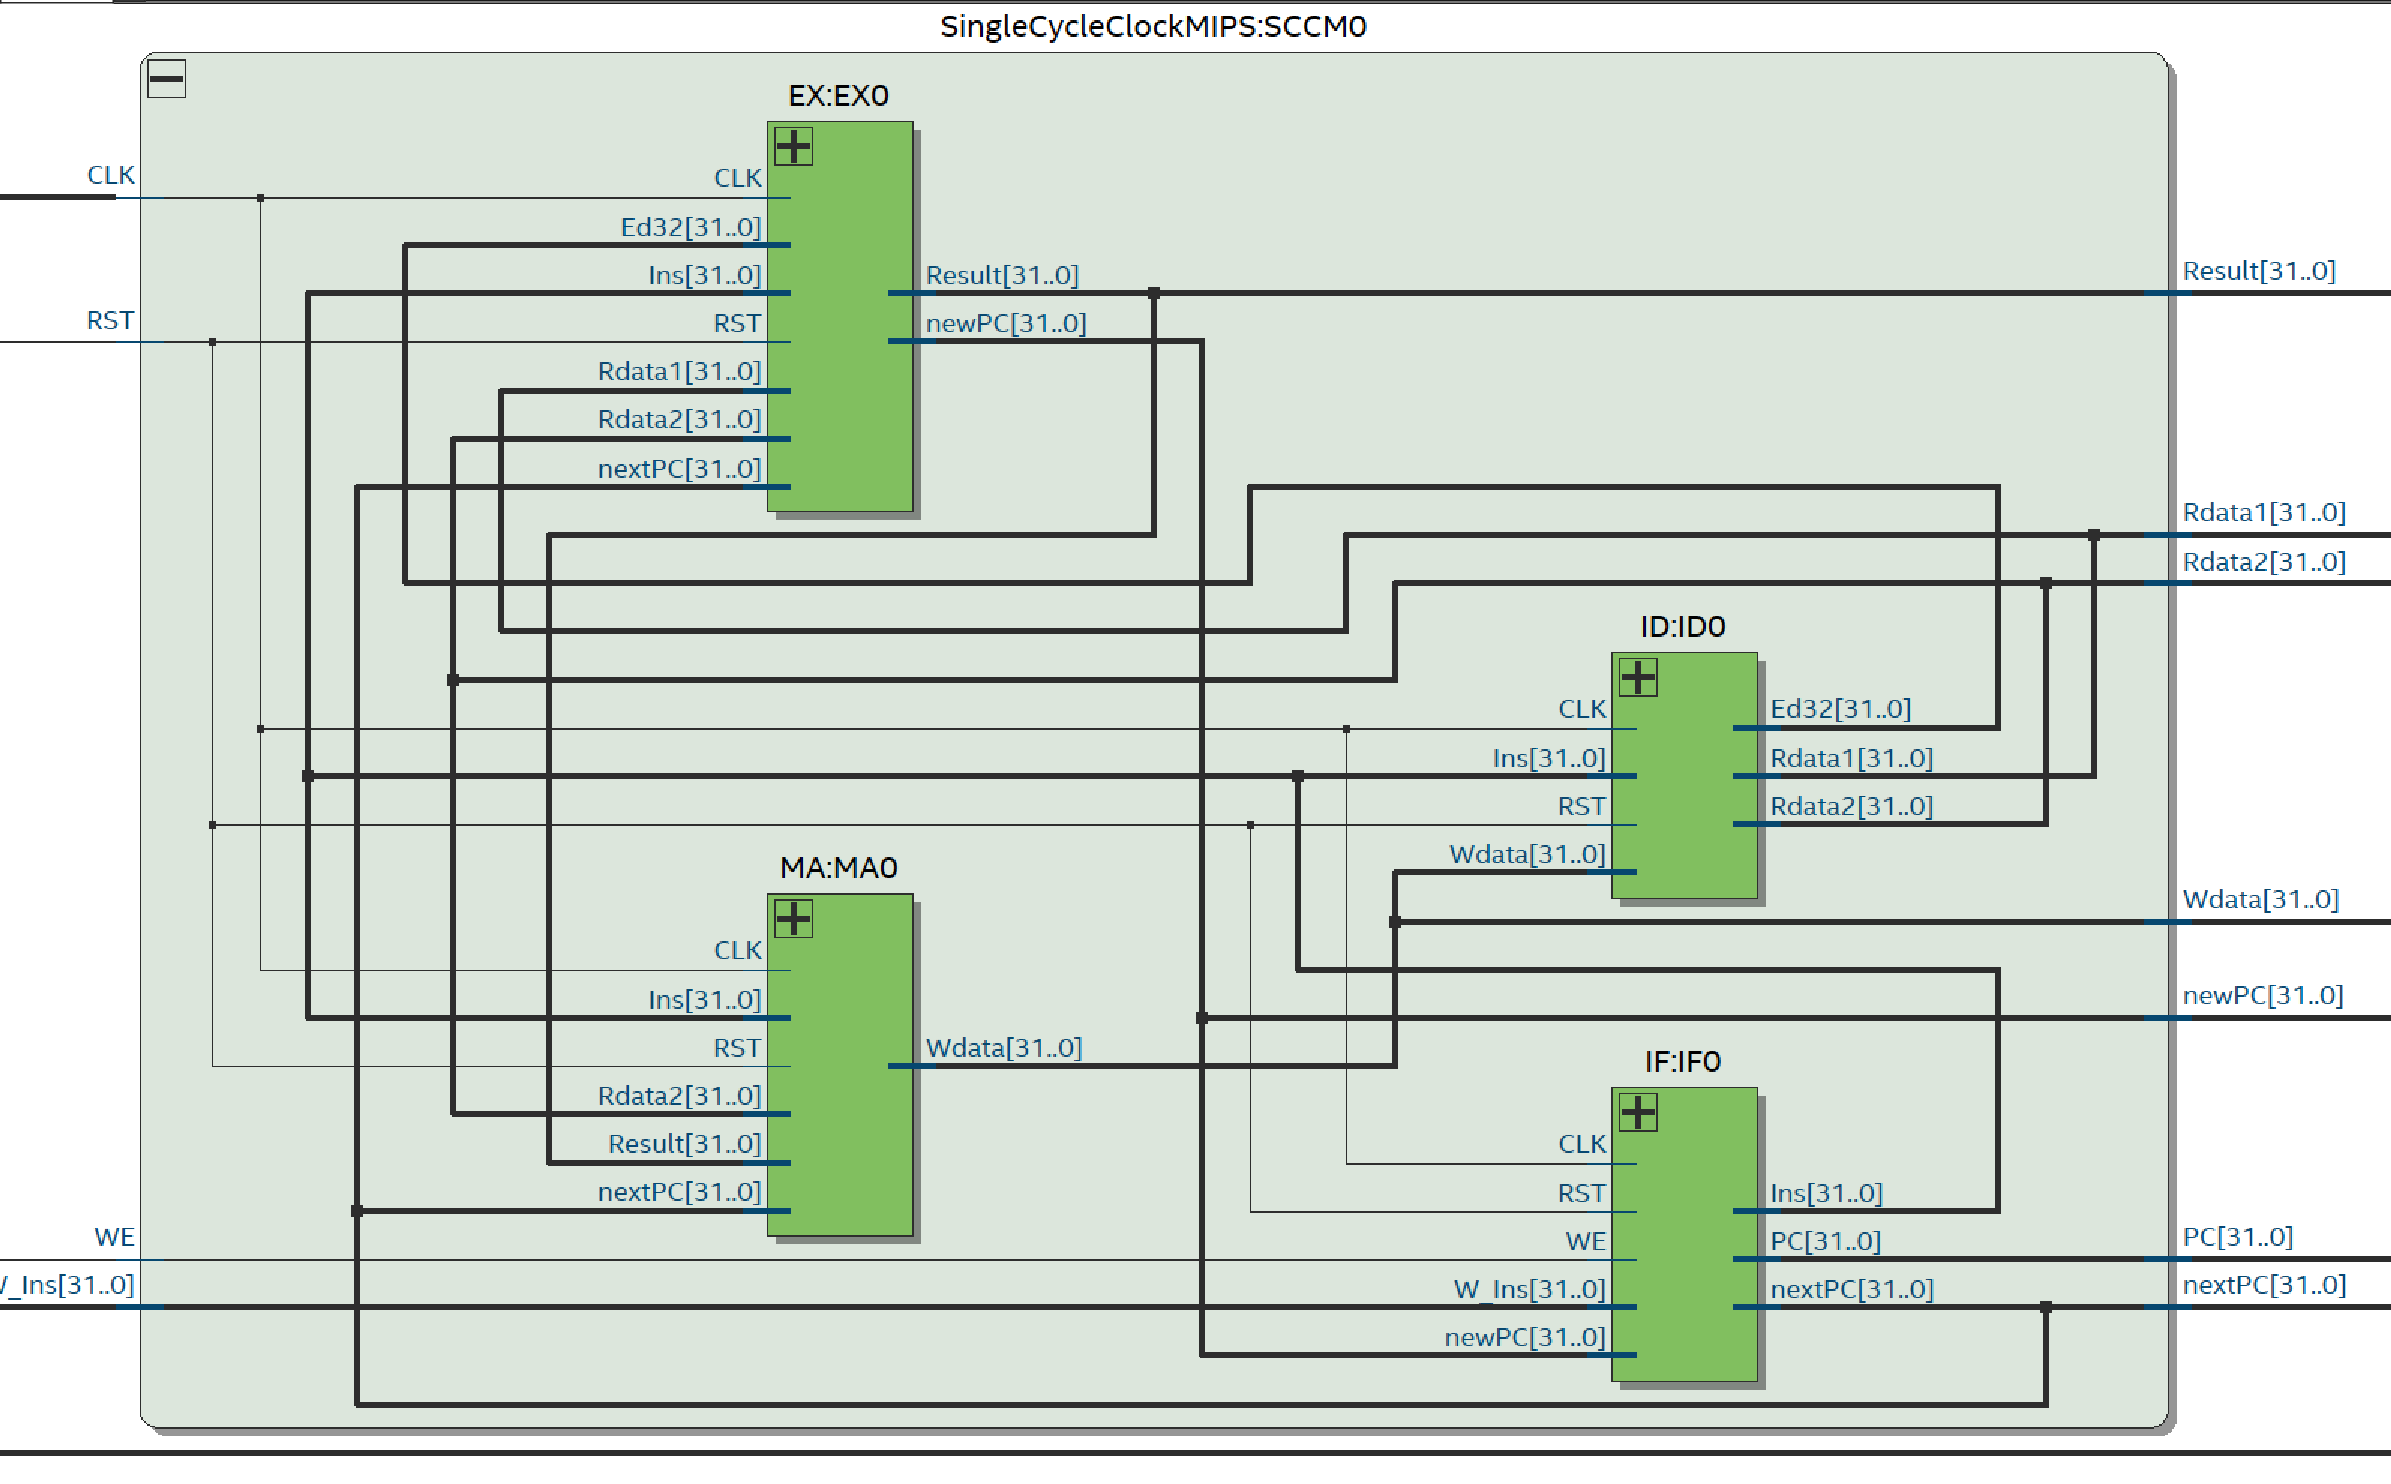
\includegraphics[width=\textwidth]{sccm.png}
  \caption{SingleCycleClockMIPS のサブモジュール接続関係}
  \label{fig:sccm_mod}
\end{figure}

本モジュールはIFモジュールを利用し,
命令メモリから命令を読み出し,
ID, EX, MAモジュールを利用し,命令を実行する.

\subsection{IF}
このモジュールはSingleCycleClockMIPS内で利用されており,
入力として与えられたプログラムカウンタ(PC)に記載された命令を読み出し,
それを\texttt{Ins}として出力する.
また,PCに4を加えた値を\texttt{nextPC}として出力する.
命令メモリの保持,読み出しにはIMモジュールを用いる.
コンパイル時に最適化され命令メモリのアドレスが変わることを防ぐため,
SW8及びGPIOの出力を入力とし,それぞれIMの入力とする.

本モジュールの入力・出力信号を表\ref{tab:if_input},\ref{tab:if_output}に示す.
\begin{table}[h]
  \caption{IF の入力}
  \centering
  \begin{tabular}{l|l|l}
    信号名 & ビット幅 & 説明 \\
    \hline
    CLK & [0:0] & SingleCycleClockMIPS 用のクロック信号 \\
    RST & [0:0] & リセット用信号 \\
    WE & [0:0] & コンパイル時にIFモジュールの最適化を防止するための信号 \\
    W\_Ins & [31:0] & コンパイル時にIFモジュールの最適化を防止するための信号 \\
    newPC & [31:0] & 次に実行する命令のアドレスを示す値 \\
  \end{tabular}
  \label{tab:if_input}
\end{table}
\begin{table}[h]
  \caption{IF の出力}
  \centering
  \begin{tabular}{l|l|l}
    信号名 & ビット幅 & 説明 \\
    \hline
    PC & [31:0] & 今から実行する命令のアドレスを示す値 \\
    nextPC & [31:0] & PC に 4 を加えた値 \\
    Ins & [31:0] & IMモジュールを用いて読み出した命令を示す値 \\
  \end{tabular}
  \label{tab:if_output}
\end{table}

本モジュールでは,IMモジュールをIM0としてインスタンス化する.

\subsection{IM}
本モジュールはIF内で利用されており,
入力として与えられたPCに記載された命令を読み出し,
Insとしてその値を出力する.
命令はワード単位であるため,PCを2ビット右シフトした値の番地から命令を読み出す.
またコンパイル時に\texttt{IMem.txt}として命令を読み出し,
最大IMEM\_SIZE個の命令をレジスタに格納する.
その他に,コンパイル時の最適化によってアドレスが変わることを防ぐため,
今回は動作することはないが,
命令メモリの書き換え信号WEが入力された場合にW\_Insの値を命令メモリ(レジスタ)に書き込む処理を加えている.

本モジュールの入力・出力信号を表\ref{tab:im_input}, \ref{tab:im_output}に示す.
\begin{table}[h]
  \caption{IMの入力}
  \centering
  \begin{tabular}{l|l|l}
    信号名 & ビット幅 & 説明 \\
    \hline
    CLK & [0:0] & SingleCycleClockMIPS 用のクロック信号 \\
    RST & [0:0] & リセット用信号 \\
    WE & [0:0] & コンパイル時にIFモジュールの最適化を防止するための信号 \\
    W\_Ins & [31:0] & コンパイル時にIFモジュールの最適化を防止するための信号 \\
    PC & [31:0] & 命令を読み出すアドレス \\
  \end{tabular}
  \label{tab:im_input}
\end{table}
\begin{table}[h]
  \caption{IM の出力}
  \centering
  \begin{tabular}{l|l|l}
    信号名 & ビット幅 & 説明 \\
    \hline
    Ins & [31:0] & 命令メモリから読み出した命令を示す値 \\
  \end{tabular}
  \label{tab:im_output}
\end{table}


\subsection{ID}
本モジュールはSingleClockCycleMIPS内で利用されており,
命令を示す値に従ってレジスタファイルから値を読み出し,
それぞれRdata1, Rdata2として出力する.
また,命令に応じて符号拡張した値をEd32として出力する.
また,レジスタファイルへの書き込み信号WEが入力された場合に,
Wdataで示された値をレジスタファイルの適切なアドレスへ書き込む.
なお,WEは命令解読によって生成する.

本モジュールの入力・出力信号を表\ref{tab:id_input}, \ref{tab:id_output}に示す.
\begin{table}[h]
  \caption{ID の入力}
  \centering
  \begin{tabular}{l|l|l}
    信号名 & ビット幅 & 説明 \\
    \hline
    CLK & [0:0] & SingleCycleClockMIPS 用のクロック信号 \\
    RST & [0:0] & リセット用信号 \\
    Ins & [31:0] & IFモジュールで読み出した命令を示す値 \\
    Wdata & [31:0] & MAモジュールで出力されるレジスタファイルへ書き込む値 \\
  \end{tabular}
  \label{tab:id_input}
\end{table}
\begin{table}[h]
  \caption{ID の出力}
  \centering
  \begin{tabular}{l|l|l}
    信号名 & ビット幅 & 説明 \\
    \hline
    Rdata1 & [31:0] & Ins[25:21]から読み出したレジスタファイルの値 \\
    Rdata2 & [31:0] & Ins[20:16]から読み出したレジスタファイルの値 \\
    Ed32 & [31:0] & Ins[15:0] を符号拡張した値 \\
  \end{tabular}
  \label{tab:id_output}
\end{table}


\subsection{EX}
本モジュールはSingleClockCycleMIPS内で利用されており,
加算や減算などの演算を行うALUと,分岐命令に応じてnewPCを決定する部分からなる.
ALUは入力されたRdata1, とRdata2, Ed32 から命令に応じて決定した片方の値を用いて演算を行う.
演算の種類はInsを用い,解読することで決定する.
また,分岐命令とジャンプ命令が読み出された場合に,
ALUの演算結果やEd32の値からnewPCを決定し,出力する.

本モジュールの入力・出力信号を表\ref{tab:ex_input}, \ref{tab:ex_output}に示す.
\begin{table}[h]
  \caption{EX の入力}
  \centering
  \begin{tabular}{l|l|l}
    信号名 & ビット幅 & 説明 \\
    \hline
    CLK & [0:0] & SingleCycleClockMIPS 用のクロック信号 \\
    RST & [0:0] & リセット用信号 \\
    Ins & [31:0] & IFモジュールで読み出した命令を示す値 \\
    Rdata1 & [31:0] & IDモジュールで読み出した値 \\
    Rdata2 & [31:0] & IDモジュールで読み出した値 \\
    Ed32 & [31:0] & IDモジュールで生成した符号拡張した値 \\
    nextPC & [31:0] & IFモジュールで生成したPCに4を加えた値 \\
  \end{tabular}
  \label{tab:ex_input}
\end{table}
\begin{table}[h]
  \caption{EX の出力}
  \centering
  \begin{tabular}{l|l|l}
    信号名 & ビット幅 & 説明 \\
    \hline
    Result & [31:0] & ALU の演算結果の値 \\
    newPC & [31:0] & 次の命令アドレスを示す値 \\
  \end{tabular}
  \label{tab:ex_output}
\end{table}

\subsection{MA}
本モジュールはSingleClockCycleMIPS内で利用されており,
データメモリ,すなわちスタック領域を扱う.
命令に応じてレジスタファイルへ書き込む値を出力するか,
入力されるRdata2で指定された値をアドレスの位置に書き込む.
命令がジャンプである場合は nextPC を出力し,
I形式算術命令またはR形式命令の場合は Resultを,
ロード命令の場合にDMモジュールを用いてデータメモリから読み出した値を出力する.

本モジュールの入力・出力信号を表\ref{tab:ma_input}, \ref{tab:ma_output}に示す.
\begin{table}[h]
  \caption{ma の入力}
  \centering
  \begin{tabular}{l|l|l}
    信号名 & ビット幅 & 説明 \\
    \hline
    CLK & [0:0] & SingleCycleClockMIPS 用のクロック信号 \\
    RST & [0:0] & リセット用信号 \\
    Ins & [31:0] & IFモジュールで読み出した命令を示す値 \\
    Result & [31:0] & EXモジュールの ALU の演算結果の値(データメモリのアドレス) \\
    Rdata2 & [31:0] & IDモジュールで読み出した値(書き込む値) \\
    nextPC & [31:0] & IFモジュールで生成したPCに4を加えた値 \\
  \end{tabular}
  \label{tab:ma_input}
\end{table}
\begin{table}[h]
  \caption{MA の出力}
  \centering
  \begin{tabular}{l|l|l}
    信号名 & ビット幅 & 説明 \\
    \hline
    Wdata & [31:0] & レジスタファイルへ書き込む値 \\
  \end{tabular}
  \label{tab:ma_output}
\end{table}

本モジュールでは,DMモジュールをDM0としてインスタンス化する.

\subsection{DM}
本モジュールは,MA内で利用されており,
データメモリを扱う.
今回はデータメモリのサイズが128であるため,
入力されたアドレスの下位7ビットのみを利用してデータメモリを示すレジスタから値を読み出す.
データメモリへの書き込みを示すWEが入力された場合は,
入力されたアドレスへ値を書き込む.

本モジュールの入力・出力信号を表\ref{tab:dm_input}, \ref{tab:dm_output}に示す.
\begin{table}[h]
  \caption{ma の入力}
  \centering
  \begin{tabular}{l|l|l}
    信号名 & ビット幅 & 説明 \\
    \hline
    CLK & [0:0] & SingleCycleClockMIPS 用のクロック信号 \\
    RST & [0:0] & リセット用信号 \\
    Adr & [31:0] & 読み出し,書き込み先アドレス ([6:0]のみ利用) \\
    WDATA & [31:0] & 書き込みデータ \\
  \end{tabular}
  \label{tab:ma_input}
\end{table}
\begin{table}[h]
  \caption{MA の出力}
  \centering
  \begin{tabular}{l|l|l}
    信号名 & ビット幅 & 説明 \\
    \hline
    Rdata & [31:0] & データメモリから読み出した値 \\
  \end{tabular}
  \label{tab:ma_output}
\end{table}

\subsection{SELECTOR}
本モジュールは Golden\_Top で利用されており,
SingleCycleClockMIPSの動作を確認するために用いる7SEGに表示するデータを出力する.
DE10-liteのSW2-0を利用し,6種類のデータを選択する.
表\ref{tab:selector}に入力パターンと選択する信号を示す.
\begin{table}
  \caption{SELECTOR の入力パターンと出力信号}
  \centering
  \begin{tabular}{l|l}
    SW2, SW1, SW0 & 出力信号 \\
    \hline
    0, 0, 0 & Rdata1 \\
    0, 0, 1 & Rdata2 \\
    0, 1, 0 & Result \\
    0, 1, 1 & Wdata \\
    1, 0, 0 & nextPC \\
    1, 0, 1 & newPC \\
  \end{tabular}
  \label{tab:selector}
\end{table}

本モジュールの入力・出力信号を表\ref{tab:sel_input}, \ref{tab:sel_output}に示す.
\begin{table}[h]
  \caption{MA の入力}
  \centering
  \begin{tabular}{l|l|l}
    信号名 & ビット幅 & 説明 \\
    \hline
    Rdata1 & [31:0] & IDモジュールで読み出した値 \\
    Rdata2 & [31:0] & IDモジュールで読み出した値 \\
    Result & [31:0] & EXモジュールのALUの演算結果 \\
    Wdata & [31:0] & IDモジュールで書き込む値 \\
    nextPC & [31:0] & PCに4を加えた値 \\
    newPC & [31:0] & 次に命令を実行するアドレス \\
  \end{tabular}
  \label{tab:ma_input}
\end{table}
\begin{table}[h]
  \caption{MA の出力}
  \centering
  \begin{tabular}{l|l|l}
    信号名 & ビット幅 & 説明 \\
    \hline
    SEL\_LED & [5:0] & 選択した信号を示すLED \\
    Vdata & [31:0] & 選択されたデータ \\
  \end{tabular}
  \label{tab:ma_output}
\end{table}

\subsection{SEG7DEC}
本モジュールは Golden\_Top で利用されており,
PCおよび,SELECTORモジュールで選択された信号を表示するために用いられる.
このモジュールは1桁のみ表示することができるため,
表\ref{tab:7seg}に示すように6個の7SEGにそれぞれ信号を振り分ける.
\begin{table}
  \caption{SEG7DEC に与える信号}
  \centering
  \begin{tabular}{l|l|l}
    DE10-lite の表示場所 & インスタンス名 & 与える信号 \\
    \hline
    HEX0 & Res00 & vdata[3:0] \\
    HEX1 & Res00 & vdata[7:4] \\
    HEX2 & Res00 & vdata[11:8] \\
    HEX3 & Res00 & vdata[15:12] \\
    HEX4 & Res00 & PC[5:2] \\
    HEX5 & Res00 & PC[9:6] \\
  \end{tabular}
  \label{tab:7seg}
\end{table}
なお,vdataはSELECTORの出力信号である.

本モジュールの入力・出力信号を表\ref{tab:7seg_input}, \ref{tab:7seg_output}に示す.
\begin{table}[h]
  \caption{SEG7DEC の入力}
  \centering
  \begin{tabular}{l|l|l}
    信号名 & ビット幅 & 説明 \\
    \hline
    DIN & [3:0] & 0--F の数値 \\
    EN & [0:0] & 値を表示するかを選択する信号 \\
    DOT & [0:0] & 7SEGのドットを表示するかを選択する信号 \\
  \end{tabular}
  \label{tab:ma_input}
\end{table}
\begin{table}[h]
  \caption{SEG7DEC の出力}
  \centering
  \begin{tabular}{l|l|l}
    信号名 & ビット幅 & 説明 \\
    \hline
    nHEX & [7:0] & 7SEGの点灯状態を示す値 \\
  \end{tabular}
  \label{tab:ma_output}
\end{table}


